\title{ALPSチュートリアル -- ALPSライブラリ}

\begin{document}

\lstset{language={C++},showspaces=false,rulecolor=\color[cmyk]{0, 0.29,0.84,0}}

\begin{frame}
  \titlepage
\end{frame}

\section*{Outline}
\begin{frame}
  \tableofcontents
\end{frame}

\section{全体構成}

\begin{frame}
  \frametitle{ALPSの階層構造}
  \begin{center}
    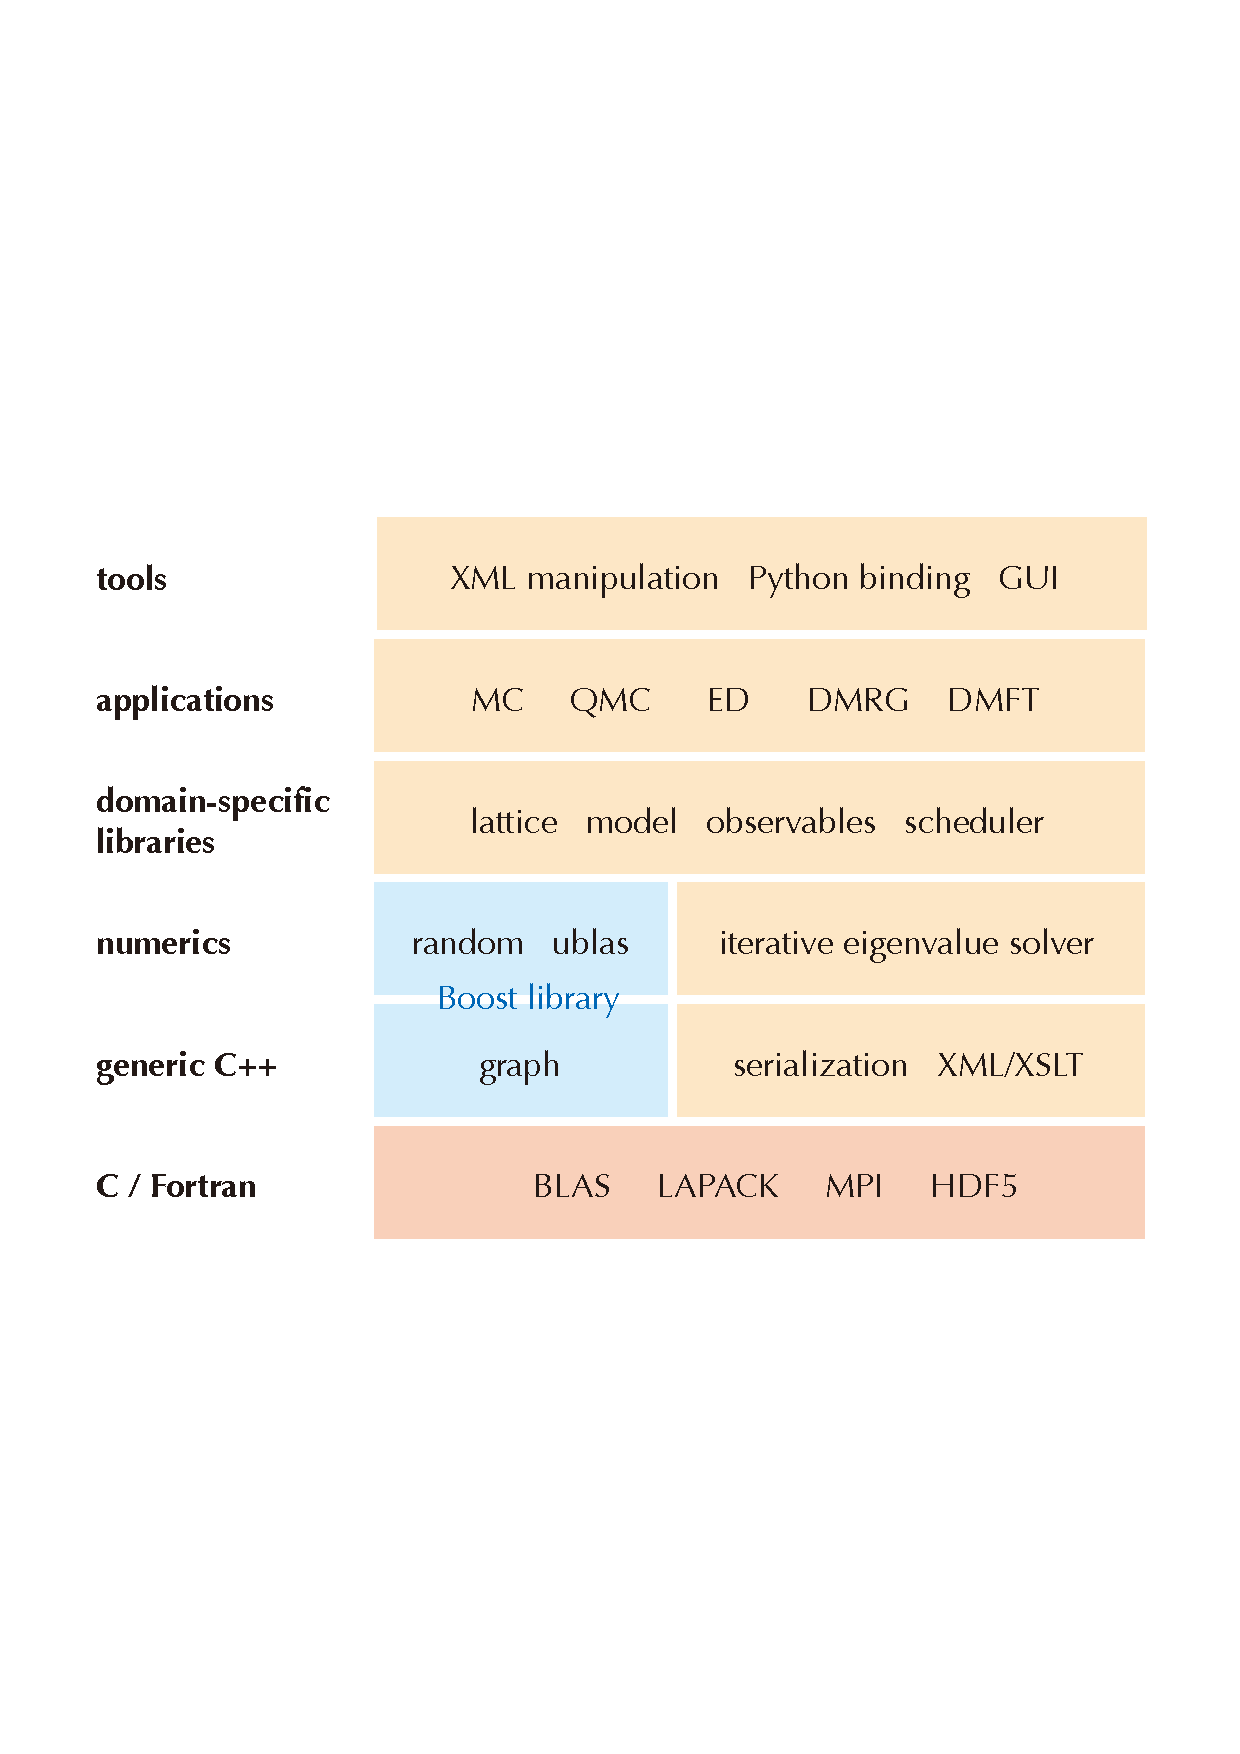
\includegraphics[height=0.65\textheight]{hierarchy.pdf}
  \end{center}
\end{frame}

\begin{frame}
  \frametitle{サードパーティーのライブラリ}
  \begin{itemize}
    \setlength{\itemsep}{1em}
  \item \href{http://www.netlib.org/blas/}{BLAS}, \href{http://www.netlib.org/lapack/}{LAPACK}: 線形演算(行列対角化、特異値分解など) (オプション)
  \item \href{http://www.mpi-forum.org/}{MPI} (Message Passing Interface): 並列計算のためのメッセージ通信 (オプション)
  \item \href{http://www.hdfgroup.org/HDF5/}{HDF5} (Hierarchical Data Format): プラットフォーム非依存のバイナリファイル格納形式
  \item \href{http://www.boost.org/}{Boost C++ Library}: 乱数, グラフ, シリアル化, など多くの有用なライブラリ群
  \end{itemize}
\end{frame}

\section{ALPS/parameter}
\begin{frame}[t,fragile]
  \frametitle{ALPS/parameterライブラリ}
  \begin{columns}[T]
    \begin{column}{.5\textwidth}
      \begin{itemize}
      \item パラメータの入出力のためのライブラリ
        %\begin{itemize}
        \item 改行, セミコロン, コンマで変数を区別
        \item 四則演算、初等関数(sin, cos, expなど)が使える
        \item $\pi$ (PI), 虚数単位(I)などを文字で指定
          \item C 風, C++風のコメント
          \item \{ \} で囲まない変数は共通パラメータ
          \item \{ \} で囲んだ変数は異なるパラメータセット
        %\end{itemize}
      \end{itemize}
    \end{column}
    \begin{column}{.5\textwidth}
    \begin{lstlisting}
LATTICE = "chain lattice";
L = 16,
SEED = 2873
// C++ style comment
SWEEPS = 4096;
THERMALIZATION = SWEEPS/8;
/* C style comment */
{ T = 2; Sq = 2*PI/3; }
{ T = 1.8; }
\end{lstlisting}
    \end{column}
  \end{columns}
\end{frame}

\begin{frame}[t,fragile]
  \frametitle{ALPS/parameterを使ったコード例}
  \lstset{language={C++}}
  \begin{lstlisting}
#include <boost/foreach.hpp>
#include <alps/parameter.h>
int main() {
  std::ifstream fin;
  fin.open("parameters.txt");
  alps::ParameterList plist(fin);
  BOOST_FOREACH(alps::Parameters& p, plist) {
    double a = p["a"];
    double b = p.value_or_default("b", 0.5);
    ...
  }
  ...
}
\end{lstlisting}
\end{frame}

\section{ALPS/alea}
\begin{frame}[t,fragile]
  \frametitle{ALPS/aleaライブラリ(1)}
  \begin{itemize}
  \item マルコフ連鎖における平均値, 分散, 自己相関を計算するライブラリ
    \lstset{language={C++}}
    \begin{lstlisting}
alps::RealObservable mag2("Magnetization^2");
...
mag2 << m * m; // in each MC step
\end{lstlisting}
  \item ビンニング解析を用いた平均値, エラー, 自己相関時間の評価
    \lstset{language={C++}}
    \begin{lstlisting}
std::cout << mag2 << std::endl;
\end{lstlisting}
  \begin{itemize}
  \item 出力
\lstset{language={bash}}
\begin{lstlisting}
Magnetization^2: 1.5 +/- 0.707; tau = inf WARNING: check error convergence
\end{lstlisting}
  \end{itemize}
  \end{itemize}
\end{frame}

\begin{frame}[t,fragile]
  \frametitle{ALPS/aleaライブラリ(2)}
  \begin{itemize}
  \item ジャックナイフ法を用いた非線形量のエラー評価
    \lstset{language={C++}}
    \begin{lstlisting}
alps::RealObsevaluator mag2eval(mag2);
alps::RealObsevaluator mag4eval(mag4);
alps::RealObsevaluator binder = mag2eval * mag2eval / mag4eval;
std::cout << binder;
\end{lstlisting}
  \begin{itemize}
  \item 出力
\lstset{language={bash}}
\begin{lstlisting}
(Magnetization^2) * (Magnetization^2) / (Magnetization^4): 0.45 +/- 0.25 WARNING: check error convergence
\end{lstlisting}
  \end{itemize}
  \end{itemize}
\end{frame}

\section{ALPS/lattice}
\begin{frame} [t,fragile,shrink]
  \frametitle{ALPS/latticeライブラリ}
  \begin{itemize}
    \setlength{\itemsep}{1em}
  \item 「格子構造」は数学的には「グラフ」で表現できる
    \begin{itemize}
    \item site $\Leftrightarrow$ vertex
    \item bond $\Leftrightarrow$ edge
    \end{itemize}
  \item Boost Graph Library に対する「ラッパー」を提供
    \begin{itemize}
    \item XMLによる「格子構造」の入出力
    \item 「ユニットセル」による繰り返し構造の指定
    \item 座標、パリティ、逆格子ベクトルなどの属性
    \end{itemize}
  \item あらかじめ用意されている格子: "chain lattice", "square lattice", "triangular lattice", "honeycomb lattice", "simple cubic lattice", など
  \item ``printgraph'' で格子のチェック
  \end{itemize}
\end{frame}

\begin{frame}[t,fragile]
  \frametitle{有限格子 + ユニットセルの埋め込み - 1}
  \begin{itemize}
  \item 格子の指定
  \begin{lstlisting}
<LATTICE name="2D" dimension="2">
  <BASIS>
    <VECTOR>   1 0 </VECTOR>
    <VECTOR> 0.5 1 </VECTOR>
  </BASIS>
</LATTICE>
\end{lstlisting}
  \end{itemize}
  \begin{center}
    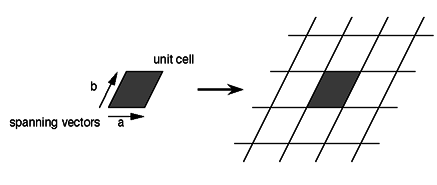
\includegraphics[height=0.3\textheight]{TutorialLatticeHOWTOLattice1}
  \end{center}
\end{frame}

\begin{frame}[t, fragile]
  \frametitle{有限格子 + ユニットセルの埋め込み - 2}
  \begin{itemize}
  \item ユニットセル
  \begin{lstlisting}
<UNITCELL name="simple1d" dimension="1" vertices="1">
  <EDGE>
    <SOURCE vertex="1" offset="0"/><TARGET vertex="1" offset="1"/>
  </EDGE>
</UNITCELL>
\end{lstlisting}
  \end{itemize}
  \begin{center}
    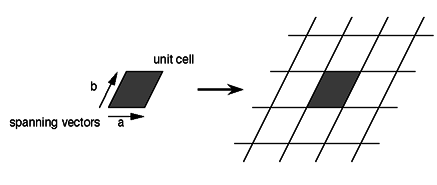
\includegraphics[height=0.3\textheight]{TutorialLatticeHOWTOLattice1}
  \end{center}
\end{frame}

\begin{frame}[t,fragile]
  \frametitle{有限格子 + ユニットセルの埋め込み - 2}
  \begin{itemize}
  \item サイズ、境界条件の指定
    \begin{lstlisting}
<LATTICEGRAPH name = "chain lattice">
  <FINITELATTICE>
    <LATTICE ref="chain lattice"/>
    <PARAMETER name="L"/>
    <EXTENT size ="L"/>
    <BOUNDARY type="periodic"/>
  </FINITELATTICE>
  <UNITCELL ref="simple1d"/>
</LATTICEGRAPH>
\end{lstlisting}
  \item より複雑な格子の作り方
    \begin{itemize}
    \item ALPS Lattice HOWTO: \url{http://alps.comp-phys.org/mediawiki/index.php/Tutorials:LatticeHOWTO}
    \end{itemize}
  \end{itemize}
\end{frame}

\section{ALPS/model}

\begin{frame}[t,fragile]
  \frametitle{ALPS/modelライブラリ}
  \begin{itemize}
%    \setlength{\itemsep}{1em}
  \item XMLを使ってハミルトニアンを定義する
    \begin{itemize}  
    \item 量子数や演算子の定義
    \item シンボリックな表現を使って, ハミルトニアンのサイト項やボンド項を定義
    \end{itemize}
    \begin{lstlisting}
Jz*Sz(i)*Sz(j)+Jxy/2*(Splus(i)*Sminus(j)+Sminus(i)*Splus(j))
\end{lstlisting}
  \item 作成した局所ハミルトニアンは行列の形で取り出せる
  \item プラケット項などのn体相互作用は難しい
  \item ALPS Model HOWTO: \url{http://alps.comp-phys.org/mediawiki/index.php/Tutorials:ModelHOWTO}
  \item あらかじめ用意されている模型: "spin", "boson Hubbard", "hardcore boson", "fermion Hubbard", "alternative fermion Hubbard", "spinless fermions", "Kondo lattice", "t-J"
  \end{itemize}
\end{frame}

\section{ALPS/scheduler}
\section{HDF5とは?}

\end{document}
